\documentclass[conference]{IEEEtran}

% ---------------------------------------------------------------
% Packages
% ---------------------------------------------------------------
\usepackage{cite}
\usepackage{amsmath,amssymb}
\usepackage{booktabs}
\usepackage{graphicx}
\usepackage{xcolor}
\usepackage{url}
\usepackage{microtype}
\usepackage{array}
\usepackage{balance}

% ---------------------------------------------------------------
% Document
% ---------------------------------------------------------------
\begin{document}

\title{Automated Zero-Trust Security Synthesis\\
for UAV SoC Architectures}

% Double-blind submission
\author{\IEEEauthorblockN{[Author names omitted for double-blind review]}}

\maketitle

% ---------------------------------------------------------------
\begin{abstract}
Autonomous UAV platforms increasingly consolidate safety-critical and
mission-critical functions onto shared System-on-Chip (SoC) hardware,
where a compromised IP core can reach every asset on the same bus
interconnect. We present an automated design space exploration (DSE)
tool that synthesizes zero-trust security architectures for UAV SoCs
using Answer Set Programming (ASP). Given an SoC topology, the tool
produces (1)~optimal security feature assignments under FPGA resource
and power constraints with solver-verified optimality, (2)~least-privilege
access control policies with mission-phase awareness, and
(3)~resilience checklists from automated fault and compromise scenarios.
An additive risk model with dual-risk budgets (security and availability)
avoids known artefacts of multiplicative ordinal-scale methods.
We evaluate on the DARPA CASE UAV surveillance architecture (11
components, 4 safety-critical), proving optimality for both max-security
and min-resources strategies. The tool identifies 22 excess privileges,
10 trust anchor gaps, and a catastrophic single-point-of-failure bus
whose loss removes 5 mission capabilities simultaneously --- findings
not surfaced by prior manual hardening of the same system.
\end{abstract}

\begin{IEEEkeywords}
Zero-Trust Architecture, UAV Security, System-on-Chip, Design Space
Exploration, Answer Set Programming
\end{IEEEkeywords}

% ---------------------------------------------------------------
\section{Introduction}

Autonomous UAV platforms are adopting SoC architectures that integrate
flight control, navigation, communications, and mission payloads onto a
single chip. This consolidation, driven by size, weight, and power (SWaP)
constraints endemic to small drones, collapses the physical isolation
that federated avionics once provided. A compromised IP core on a
shared bus can potentially reach every other component on the same
interconnect.

Zero-Trust Architecture (ZTA), as defined by NIST SP~800-207~\cite{nist_zta},
eliminates implicit trust based on network location. The FAA has mandated
ZTA transition for ground infrastructure~\cite{faa_zt}, and recent work
has called for extending ZTA to airborne systems~\cite{ztas_dasc}. However,
applying ZTA to SoC interconnects presents unique challenges: hardware
resource constraints (LUTs, flip-flops, power budgets), real-time
requirements, and the need to co-optimize security feature selection with
enforcement placement and access policy synthesis.

This paper presents an automated DSE workflow that addresses these
challenges. Using ASP with the Clingo solver, the tool takes an SoC
architectural model and produces three deliverables:
\begin{enumerate}
\item \textbf{Optimal security architectures} --- feature assignments
  minimizing residual risk under FPGA resource and power caps, with
  solver-verified optimality.
\item \textbf{Access control policies} --- least-privilege ACLs with
  three-mode security postures (normal, attack-suspected,
  attack-confirmed).
\item \textbf{Resilience checklists} --- automated fault/compromise
  scenarios with blast radius, capability loss, and attack path analysis.
\end{enumerate}

We evaluate the workflow on the DARPA CASE UAV surveillance
architecture~\cite{darpa_case}, the same system hardened manually by
Hasan et~al.~\cite{hasan_saecps} using AADL-based ZT patterns. Our
automated approach explores the full $3^{11}$ design space, proves
optimality for both optimization strategies, and surfaces privilege,
trust-boundary, and topology findings invisible to the manual method.
A secondary case study on an 8-component SoC drone confirms generality.

% ---------------------------------------------------------------
\section{Risk Model and DSE Formulation}

\subsection{SoC Graph Model}
We model the SoC as a directed graph $G=(V,E)$ with typed vertices:
bus masters $V_M$, receiver IP cores $V_R$, bus interconnects $V_B$,
firewalls (Policy Enforcement Points) $V_{FW}$, and policy servers
(Policy Decision Points) $V_{PS}$. Each component carries trust-domain,
CIA-impact, and exploitability annotations.

\subsection{Risk Equation}
For each component $c$ with asset $a$ and action
$\mathit{op} \in \{\mathit{read}, \mathit{write}, \mathit{avail}\}$:
\begin{equation}
R(c,a,\mathit{op}) = \max\!\bigl(0,\;\mathit{Imp}+\mathit{DB}+\mathit{EM}
  -\mathit{EP}-\mathit{LP}\bigr)
\label{eq:risk}
\end{equation}
where $\mathit{Imp}$ is CIA impact (1--5), $\mathit{DB}\in[0,3]$ is a
trust-domain bonus (low-trust components receive higher base risk),
$\mathit{EM}$ offsets from median CVSS~v3.1 attack complexity for SoC IP
cores, $\mathit{EP}$ is the protection value of the assigned security
feature, and $\mathit{LP}$ is the logging detection capability. This
additive formulation avoids the artefacts Aven~\cite{aven_riskmatrix}
identified in multiplicative risk matrices on ordinal scales, and aligns
with NIST SP~800-30~\cite{nist_sp80030}.

\subsection{Dual-Risk Budget}
Two independent hard constraints replace a single risk cap:
(1)~a \emph{security risk budget} bounds $R(c,a,\mathit{op})$ for
non-redundant components; (2)~an \emph{availability risk budget} bounds
combined failure probability for redundancy-group members. This
separation enables independent optimization of feature selection and
redundancy architecture.

\subsection{Three-Phase Workflow}
The solver assigns exactly one security feature and one logging feature
per component from a catalog with Vivado post-implementation resource
estimates (PYNQ-Z2 target), minimizing weighted risk subject to LUT,
flip-flop, and power caps. Phase~2 synthesizes firewall/policy-server
placement with least-privilege analysis and mode-aware access control.
Phase~3 auto-generates fault and compromise scenarios computing
blast radius, capability loss, and attack paths.

% ---------------------------------------------------------------
\section{DARPA CASE UAV Evaluation}

\begin{figure}[t]
  \centering
  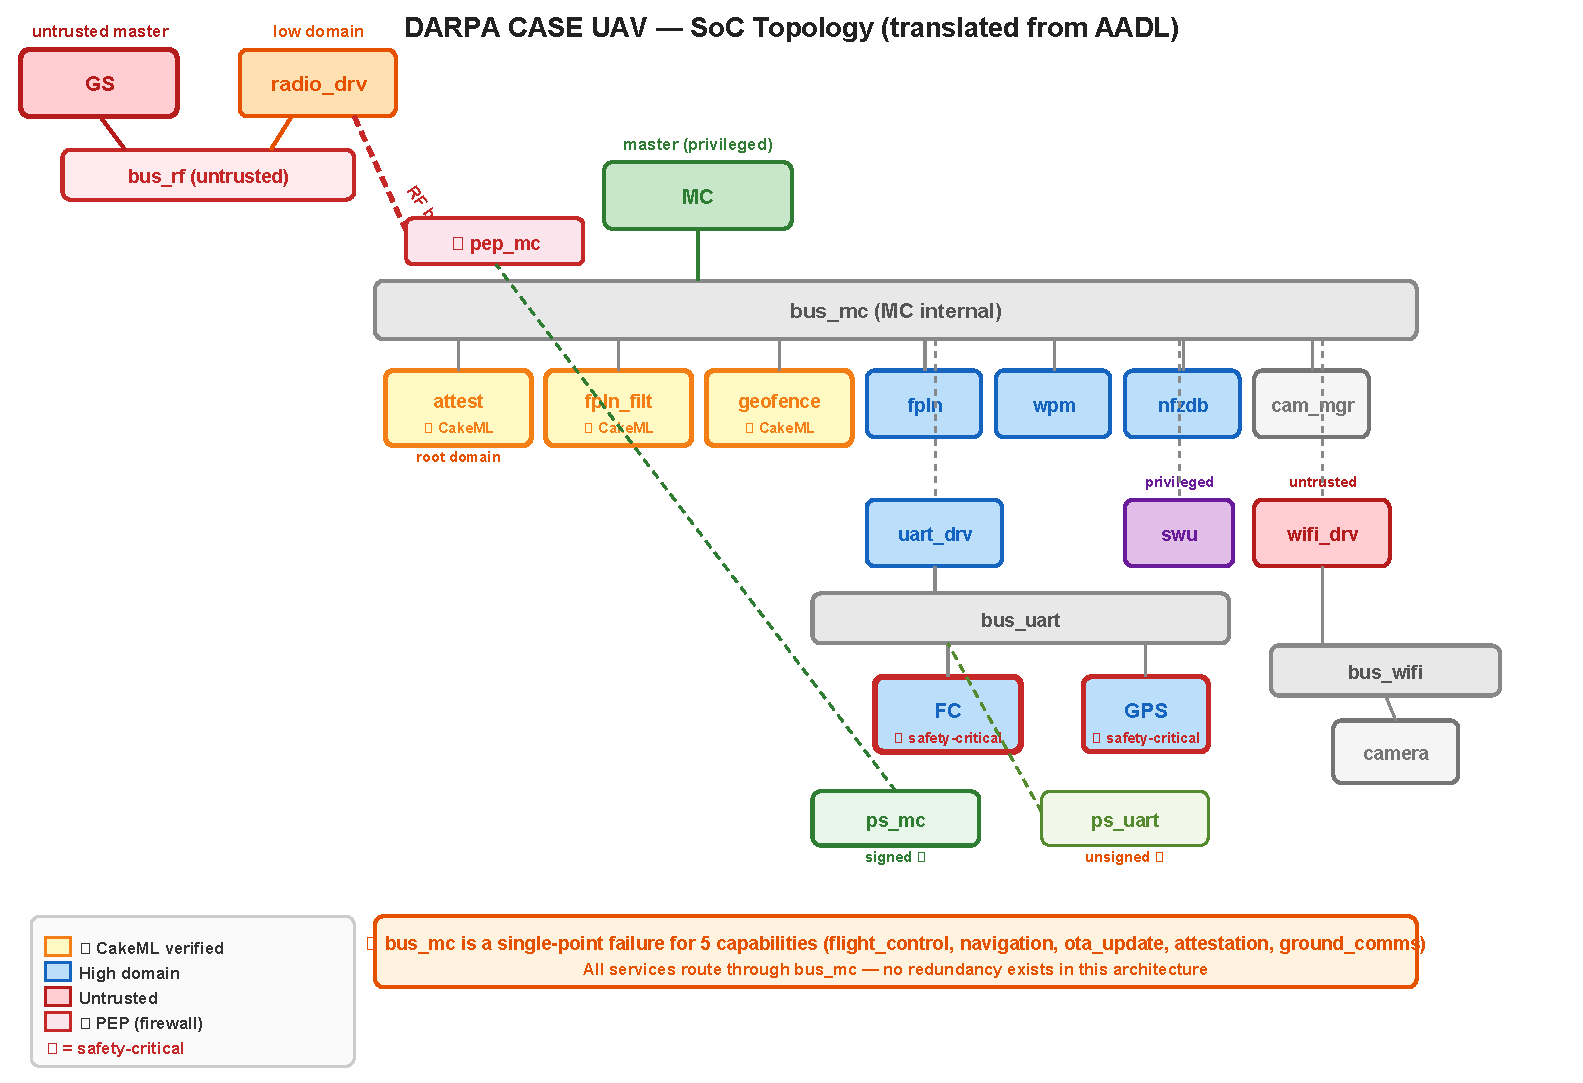
\includegraphics[width=\columnwidth]{fig4_darpa_uav_topology}
  \caption{DARPA CASE UAV SoC topology translated from AADL.
    The ground station (gs, untrusted) reaches the trusted MC bus
    via radio\_drv --- the primary attack vector. All services
    route through bus\_mc, creating a single-point availability failure.}
  \label{fig:uav}
\end{figure}

We translated the DARPA CASE UAV surveillance architecture --- the
system used by Hasan et~al.~\cite{hasan_saecps} to demonstrate manual
ZT pattern application --- from its AADL software model into our SoC
interconnect representation (Fig.~\ref{fig:uav}). The architecture has
11~receivers across 4~buses, 3~masters, 4~safety-critical components,
and zero redundancy groups. Three BriefCASE/Collins hardening additions
(attestation gate, flight plan filter, geofence monitor) are modeled
as CakeML-verified components with exploitability~=~1.

\subsection{Phase~1: Security Feature Optimization}

Under \textbf{max\_security} (proven optimal in 15.5~s),
zero\_trust$+$zt\_logger is assigned to 8 of 11 components, achieving
total weighted risk~=~0 at 34\% LUT utilization (18,170/53,200~LUTs,
367~mW). CakeML-verified components achieve risk~=~0 without dominating
the resource budget.

Under \textbf{min\_resources}, a progressive-timeout continuation run
proved optimality after 6~attempts totaling 63~minutes
(Table~\ref{tab:convergence}). The proven-optimal solution assigns
\texttt{mac} to all 11~components with selective logging, achieving
risk~=~39 at 15\% LUTs (8,410/53,200) and 160~mW --- a \textbf{54\% LUT
reduction} versus max\_security for a risk increase from 0 to~39.

\begin{table}[t]
\caption{UAV min\_resources Progressive-Timeout Convergence}
\label{tab:convergence}
\centering
\scriptsize
\begin{tabular}{rrrrrrl}
\toprule
Att. & Timeout & Models & Risk & LUTs & mW & Status \\
\midrule
1 &   60\,s & 15 & 31 & 10{,}240 & 198 & best-found \\
2 &  120\,s & 10 & 34 &  9{,}380 & 180 & best-found \\
3 &  300\,s &  4 & 38 &  9{,}130 & 174 & best-found \\
4 &  600\,s &  8 & 39 &  8{,}410 & 160 & best-found \\
5 & 1200\,s &  0 & 39 &  8{,}410 & 160 & no improve \\
6 & 1800\,s &  0 & 39 &  8{,}410 & 160 & \textbf{optimal} \\
\bottomrule
\end{tabular}
\end{table}

The convergence profile is notable: initial attempts aggressively
reduce risk (overshooting on resources), and subsequent attempts
monotonically trade risk for resources until the Pareto frontier is
reached. Attempt~5 finds no improvement; attempt~6 exhausts the
remaining search space and proves optimality. This progressive-timeout
strategy is essential for UAV-scale problems where a single long
timeout would waste budget on already-explored regions.

\subsection{Phase~2: ZTA Policy Synthesis}

The solver placed 1~firewall (pep\_mc) and 1~policy server (ps\_uart),
then identified \textbf{22 excess privileges}: the ground station (gs,
untrusted) holds topological access to all 9~MC-bus components via
radio\_drv while requiring only radio\_drv read$+$write (10\% policy
tightness). Trust anchor analysis found 10~components lacking hardware
root of trust, 2~unattested masters, and 1~unsigned policy server.

\subsection{Phase~3: Resilience and SPOF Discovery}

Twenty-four scenarios were generated. Under max\_security all scenario
risks are~0 (base risk~0). Under min\_resources, worst-case
2.06$\times$ amplification under ps\_uart compromise.

The critical finding: \texttt{bus\_mc} failure loses \textbf{5
capabilities simultaneously} --- flight control, navigation, OTA update,
attestation, and ground communications. This single-point-of-failure is
a topology-level vulnerability that \emph{no security feature assignment
can mitigate}; it requires architectural redesign (bus replication or
cross-connect). This finding was not surfaced by the manual AADL-based
hardening approach applied to the same system.

\subsection{Comparison with Manual Hardening}

Table~\ref{tab:comparison} compares the automated tool with the manual
AADL ZT pattern approach of Hasan et~al.~\cite{hasan_saecps,hasan_jsys}
on the same UAV architecture. The two operate at different abstraction
levels --- software architecture with CakeML on seL4 vs.\ hardware
interconnect topology --- so this comparison is portability evidence
rather than a strict tool-vs-tool evaluation.

\begin{table}[t]
\caption{Automated DSE vs.\ Manual AADL Hardening (Same UAV)}
\label{tab:comparison}
\centering
\scriptsize
\setlength{\tabcolsep}{3pt}
\begin{tabular}{lll}
\toprule
Dimension & Collins/Hasan~\cite{hasan_saecps} & This Tool \\
\midrule
Method    & Manual pattern selection & Constraint-solving DSE \\
Optimality& Not verified & Proven (both strategies) \\
Privilege & Not in scope & 22 excess flagged \\
SPOF      & Not surfaced & bus\_mc: 5-cap loss \\
Resources & Not quantified & 15--34\% LUT range \\
\bottomrule
\end{tabular}
\end{table}

% ---------------------------------------------------------------
\section{Implementation}

The tool comprises 13,701 lines across 33 files: 15~ASP encodings,
8~Python core modules, 4~phase orchestrators, 5~GUI modules, and a
Vivado IP catalog providing Xilinx Zynq-7000 (PYNQ-Z2, xc7z020clg400-1)
post-implementation resource estimates. Phase solve times: Phase~1
$<$5\,s (SoC drone) / 15.5\,s (UAV max\_security); Phase~2 $<$2\,s;
Phase~3 $<$30\,s for 18--24 scenarios. The orchestrator runs three
optimization strategies (max\_security, min\_resources, balanced) in
parallel. Input modes include built-in factory models and a
drag-and-drop network editor with JSON save/load and ASP export. The
tool is available as open-source software [URL redacted for
double-blind review].

% ---------------------------------------------------------------
\section{Secondary Case Study: SoC Drone}

To confirm generality, we applied the tool to an 8-component SoC drone
(TC9) with 2~bus masters, 2~NoC buses, a 5-member redundancy group,
and 1~safety-critical component. All three strategies (max\_security,
min\_resources, balanced) achieved solver-verified optimality in under
9~seconds. The tool identified 9~excess privileges, 6~trust anchor
gaps, and a 3.0$\times$ worst-case risk amplification from policy-server
compromise. The redundancy group exercises the dual-risk budget
(security vs.\ availability) absent in the non-redundant UAV. Together,
the two cases demonstrate the workflow's applicability to both redundant
and non-redundant UAV/drone topologies.

% ---------------------------------------------------------------
\section{Related Work}

Hardware-enforced SoC isolation (ARM TrustZone~\cite{arm_tz}, Xilinx
isolation design flow~\cite{xilinx_idf}) provides static partitioning
but does not optimize feature placement under resource constraints.
The DARPA CASE program~\cite{darpa_case} produced the BriefCASE toolchain
for AADL model transformations with CakeML-verified components on seL4;
Hasan et~al.~\cite{hasan_saecps,hasan_jsys} defined ZT patterns and
applied them manually to the UAV we evaluate. Their stated future work
is to build automated tooling for ZT-compliant CPS design-time
assurance --- the objective this paper addresses through constraint
solving. ASP~\cite{gebser_asp} provides exact optimization with
constraint-satisfaction guarantees that heuristic methods (NSGA-II,
genetic algorithms) cannot offer.

% ---------------------------------------------------------------
\section{Conclusion}

This paper presented an automated DSE workflow that synthesizes
zero-trust security architectures for UAV SoC platforms. On the DARPA
CASE UAV, the tool proves optimality for both max-security (risk~=~0,
34\% LUT) and min-resources (risk~=~39, 15\% LUT) strategies, identifies
22~excess privileges and 10~trust anchor gaps, and discovers a
catastrophic bus SPOF invisible to prior manual hardening. A
progressive-timeout continuation strategy enables proven optimality
for 11-component problems within practical wall-clock time (63~min).
The central conclusion is that UAV SoC security should be treated as a
constrained architecture-synthesis problem amenable to formal
optimization, not a manual hardening exercise.

Future work includes runtime-adaptive mode transitions driven by anomaly
scoring, latency-aware constraint modeling for real-time UAV control
loops, multi-chip topology support, and integration with DO-326A
certification evidence generation~\cite{do326a}.

% ---------------------------------------------------------------
\balance
\bibliographystyle{IEEEtran}
\bibliography{dsas_references}

\end{document}
